% This file was created by matlab2tikz.
%
%The latest updates can be retrieved from
%  http://www.mathworks.com/matlabcentral/fileexchange/22022-matlab2tikz-matlab2tikz
%where you can also make suggestions and rate matlab2tikz.
%
\definecolor{mycolor1}{rgb}{0.00000,0.44700,0.74100}%
\definecolor{mycolor2}{rgb}{0.85000,0.32500,0.09800}%
%
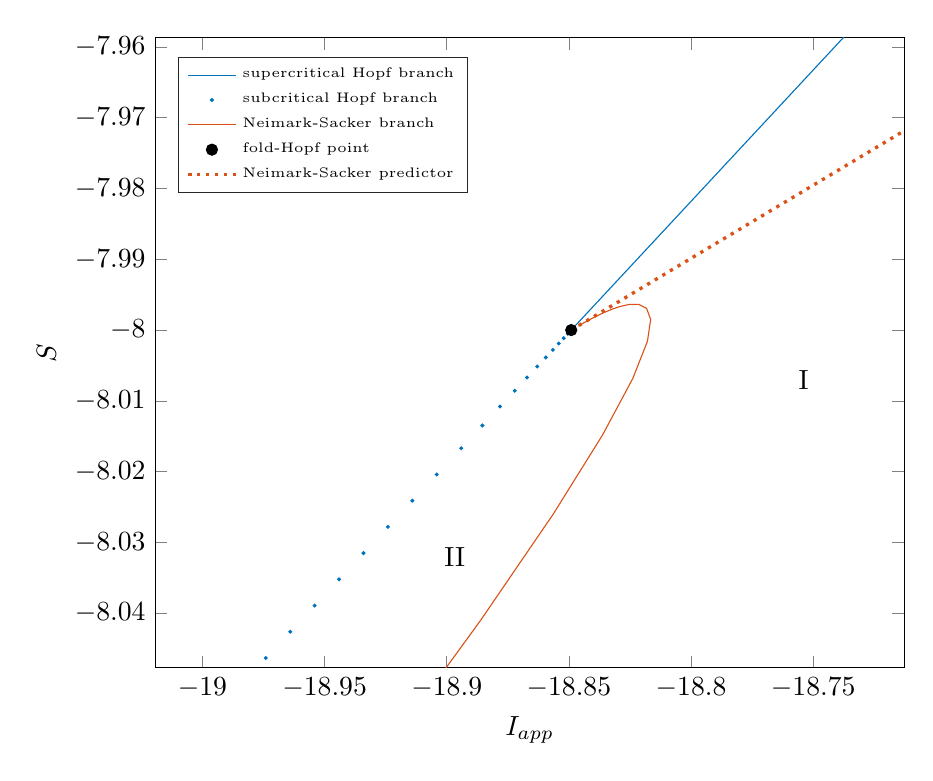
\begin{tikzpicture}[%
mark size=0.5
]

\begin{axis}[%
width=9.509cm,
height=8cm,
at={(0cm,0cm)},
scale only axis,
xmin=-19.0193,
xmax=-18.7128,
xlabel={$I_{app}$},
ymin=-8.0477,
ymax=-7.9587,
ylabel={$S$},
axis background/.style={fill=white},
legend style={at={(0.03,0.97)},anchor=north west,legend cell align=left,align=left,draw=white!15!black,font=\tiny},
]
\addplot [color=mycolor1,solid]
  table[row sep=crcr]{%
-18.8473611635171	-7.99937663262835\\
-18.8453435786192	-7.99862857396533\\
-18.8429224616458	-7.99773087791389\\
-18.8400170995462	-7.99665360570904\\
-18.8365306337442	-7.99536082586726\\
-18.8323468297544	-7.99380941345869\\
-18.8273262001602	-7.99194760827308\\
-18.8213013513833	-7.98971328323613\\
-18.8140713986497	-7.98703186451844\\
-18.8053952622902	-7.98381383280051\\
-18.7953950012695	-7.98010432648132\\
-18.7853947220817	-7.97639443995615\\
-18.7753944432488	-7.97268418006628\\
-18.7653941647705	-7.96897354678254\\
-18.7553938866461	-7.96526254007558\\
-18.745393608875	-7.96155115991597\\
-18.7353933314566	-7.95783940627421\\
};
\addlegendentry{supercritical Hopf branch};

\addplot [color=mycolor1,only marks,mark=*,mark options={solid}]
  table[row sep=crcr]{%
-18.9840827111782	-8.0500334008489\\
-18.974082996765	-8.04633076532673\\
-18.9640832819851	-8.0426277567487\\
-18.9540835668391	-8.0389243750874\\
-18.9440838513277	-8.03522062031534\\
-18.9340841354515	-8.03151649240495\\
-18.9240844192113	-8.0278119913286\\
-18.9140847026077	-8.02410711705855\\
-18.9040849856415	-8.0204018695671\\
-18.8940852495942	-8.01669624188913\\
-18.8854110644888	-8.01348152477592\\
-18.8781824145905	-8.01080231919396\\
-18.8721584270594	-8.00856945716304\\
-18.8671383593024	-8.00670860637588\\
-18.862954915269	-8.00515780542915\\
-18.8594686742633	-8.00386540745132\\
-18.8565634472944	-8.00278836479449\\
-18.8541424066802	-8.00189079845536\\
-18.8521248602416	-8.00114280512363\\
-18.8504435627995	-8.00051946249868\\
-18.8490424755272	-8\\
};
\addlegendentry{subcritical Hopf branch};

\addplot [color=mycolor2,solid]
  table[row sep=crcr]{%
-18.8459115709366	-7.99935308932846\\
-18.8458486397543	-7.99934008642396\\
-18.8458576513713	-7.99935603238597\\
-18.8457656904585	-7.99933793282778\\
-18.8456534624642	-7.99931581238519\\
-18.8455166588289	-7.99928890095464\\
-18.8453493923559	-7.99925606341499\\
-18.8451444700395	-7.99921596927426\\
-18.8448925098043	-7.9991668556351\\
-18.8445816185486	-7.99910653110832\\
-18.8441967352125	-7.99903229819759\\
-18.8437184686802	-7.99894074773913\\
-18.8431220516601	-7.99882767524791\\
-18.8423762170227	-7.99868807492233\\
-18.8414414391827	-7.998516036531\\
-18.8402691216081	-7.9983051720946\\
-18.8388008259952	-7.9980492762703\\
-18.8369707957847	-7.99774446377785\\
-18.834711688481	-7.9973927506293\\
-18.831971949015	-7.99701011473483\\
-18.8287445663305	-7.99663864424\\
-18.8251263980072	-7.9963690694046\\
-18.8214077013447	-7.99637186500806\\
-18.8181977515604	-7.99693617787841\\
-18.8165292612146	-7.9984932508998\\
-18.8178523294519	-8.00159554119081\\
-18.823842239296	-8.00683891254281\\
-18.836160211764	-8.01478975865268\\
-18.8563634998908	-8.02597739615432\\
-18.8860175015678	-8.04094920663381\\
-18.9189967184836	-8.0566\\
};
\addlegendentry{Neimark-Sacker branch};

\addplot [color=black,mark size=2.0pt,only marks,mark=*,mark options={solid}]
  table[row sep=crcr]{%
-18.8490424755272	-8\\
};
\addlegendentry{fold-Hopf point};

\addplot [color=mycolor2,dotted,line width=1.2pt]
  table[row sep=crcr]{%
-18.8490424755272	-8\\
-18.8490105307808	-7.99999339954421\\
-18.8489146965418	-7.99997359817686\\
-18.84875497281	-7.99994059589793\\
-18.8485313595855	-7.99989439270743\\
-18.8482438568682	-7.99983498860536\\
-18.8478924646583	-7.99976238359172\\
-18.8474771829556	-7.99967657766651\\
-18.8469980117602	-7.99957757082973\\
-18.8464549510721	-7.99946536308137\\
-18.8458480008913	-7.99933995442145\\
-18.8451771612178	-7.99920134484995\\
-18.8444424320515	-7.99904953436689\\
-18.8436438133926	-7.99888452297225\\
-18.8427813052409	-7.99870631066604\\
-18.8418549075965	-7.99851489744826\\
-18.8408646204594	-7.99831028331891\\
-18.8398104438295	-7.99809246827799\\
-18.838692377707	-7.9978614523255\\
-18.8375104220917	-7.99761723546143\\
-18.8362645769837	-7.9973598176858\\
-18.834954842383	-7.99708919899859\\
-18.8335812182896	-7.99680537939982\\
-18.8321437047035	-7.99650835888947\\
-18.8306423016246	-7.99619813746755\\
-18.829077009053	-7.99587471513406\\
-18.8274478269887	-7.995538091889\\
-18.8257547554317	-7.99518826773237\\
-18.823997794382	-7.99482524266417\\
-18.8221769438396	-7.99444901668439\\
-18.8202922038044	-7.99405958979305\\
-18.8183435742765	-7.99365696199013\\
-18.8163310552559	-7.99324113327565\\
-18.8142546467426	-7.99281210364959\\
-18.8121143487366	-7.99236987311196\\
-18.8099101612378	-7.99191444166276\\
-18.8076420842464	-7.99144580930199\\
-18.8053101177622	-7.99096397602965\\
-18.8029142617853	-7.99046894184574\\
-18.8004545163157	-7.98996070675025\\
-18.7979308813533	-7.9894392707432\\
-18.7953433568983	-7.98890463382457\\
-18.7926919429505	-7.98835679599438\\
-18.78997663951	-7.98779575725261\\
-18.7871974465768	-7.98722151759927\\
-18.7843543641509	-7.98663407703436\\
-18.7814473922323	-7.98603343555788\\
-18.7784765308209	-7.98541959316983\\
-18.7754417799168	-7.98479254987021\\
-18.7723431395201	-7.98415230565901\\
-18.7691806096305	-7.98349886053625\\
-18.7659541902483	-7.98283221450191\\
-18.7626638813734	-7.98215236755601\\
-18.7593096830057	-7.98145931969853\\
-18.7558915951453	-7.98075307092948\\
-18.7524096177923	-7.98003362124886\\
-18.7488637509464	-7.97930097065667\\
-18.7452539946079	-7.97855511915291\\
-18.7415803487767	-7.97779606673758\\
-18.7378428134527	-7.97702381341067\\
-18.734041388636	-7.9762383591722\\
-18.7301760743266	-7.97543970402215\\
-18.7262468705245	-7.97462784796053\\
-18.7222537772297	-7.97380279098735\\
-18.7181967944421	-7.97296453310259\\
-18.7140759221619	-7.97211307430626\\
-18.7098911603889	-7.97124841459836\\
};
\addlegendentry{Neimark-Sacker predictor};

\node[right, align=left, text=black]
at (axis cs:-18.76,-8.007) {I};
\node[right, align=left, text=black]
at (axis cs:-18.905,-8.032) {II};
\end{axis}
\end{tikzpicture}%